\documentclass[12pt, a4paper]{article}
\setcounter{section}{-1}
\usepackage{amsmath}
\usepackage{graphicx}
\usepackage{pythonhighlight}
\usepackage{pdflscape}

\newtheorem{theorem}{Theorem}[section]
\newtheorem{corollary}{Corollary}[theorem]
\newtheorem{lemma}[theorem]{Lemma}

\title{Numerical analysis\\
	\large Coursework 2}
\author{Stefan A. Obada \\ \textit{so1118}}
\date{March 2020}
\setcounter{secnumdepth}{0}

\begin{document}
\maketitle

\begin{abstract}
This paper solves the questions from the $2^{nd}$ Coursework. I study a recurrence relation for the $p^{th}$ derivative of Chebyshev polynomials and solve the differential equation $\ddot{y}(x)-xy(x)=0$ using this result.
Please refer to (\footnote{https://github.com/stefan-obada/chebyshev-poly}) for full documentation.

\tableofcontents
\end{abstract}

\newpage

\section{Problem 1}
\textbf{Definition:} Chebyshev polynomials are defined by the relation 
\begin{equation}
T_{n}(x) = cos(n*arccos(x))
\label{equation:def}
\end{equation}
\textbf{Note:} We use this definition, as in the lectures. However, this is just one of the 2 forms of Chebyshev polynomials. Moreover, this one holds only for \\ $x \in [-1,1]$, but we will work just with the open interval.

\subsection{Recurrence for derivatives}
To derive a recurrence relation for the $p^{th}$ derivative we will firstly derive the differential equation that is verified by $T_{n}$ and we will proceed by using Leibniz Lemma of differentiation.\vspace{4.0mm} \\
\textbf{Lemma 1:} $T_{k}$ verifies one of the Sturm-Liouville differential equations, which is:
\begin{equation}
	(1-x^2)\ddot{T_{k}}(x) = k^2T_{k}(x) + x\dot{T_{k}}(x)
\label{equation:diff}
\end{equation}
\textbf{Proof:} Differentiate $T_{k}(x)$ to obtain:
\begin{equation}
	\dot{T_{k}}(x) = k\cdot\frac{sin(k \cdot arccos(x))}{\sqrt{1-x^2}}
\label{equation:T_dot}
\end{equation}

\begin{equation*}
\begin{split}
	\ddot{T_{k}}(x) & = \frac{d}{dx}\dot{T_{k}}(x) = k \cdot \frac{cos(k \cdot arccos(x))\frac{k\sqrt{1-x^2}}{\sqrt{1-x^2}} - sin(k \cdot arccos(x)) \cdot \frac{-2x}{2\sqrt{1-x^2}}}{(1-x^2)} = \\
	& = \frac{k^2T_{k}(x) + x\dot{T_{k}}(x)}{1-x^2} \Rightarrow \underline{(1-x^2)\ddot{T_{k}}(x) = k^2T_{k}(x) + x\dot{T_{k}}(x)}
\end{split}
\end{equation*}
\vspace{4.0mm}\\
\textbf{Lemma 2:} (Leibniz formula) For $f$ and $g$ real functions n times differentiable, we have:
\begin{equation*}
	(fg)^{(n)}=\sum_{k=0}^{n}{{{n} \choose {k}} \cdot f^{(n-k)}g^{(k)}}
\end{equation*}
\textbf{Lemma 3:} The recurrence relation between the derivatives of $T=T_{n}(x)$ is given by:
\begin{equation}
	(1-x^2)T^{(p)} = (2p-3) \cdot xT^{(p-1)} + [k^2 + (p-2)^2] \cdot T^{(p-2)}
\label{equation:rec}
\end{equation}
\textbf{Proof:}
Firstly, differentiate (\ref{equation:diff}) from \textbf{Lemma 1}, $p-2$ times. Note that all the terms involved are infinite times differentiable.
\begin{equation}
[(1-x^2)\ddot{T}]^{(p-2)} = k^2T^{(p-2)} + {[x\dot{T}]}^{(p-2)}
\label{equation:p-2}
\end{equation}
We proceed by applying \textbf{Lemma 2} on LHS and RHS. Note that $(1-x^2)^{(p)}=0, \forall p\geq 3 $ and $x^{(p)}=0, \forall p\geq 2 $.
\begin{equation*}
\begin{split}
	[(1-x^2)\ddot{T}]^{(p-2)} & = {{p-2}\choose{0}}(1-x^2)T^{(p)} + {{p-2}\choose{1}}(-2x)T^{(p-1)} + {{p-2}\choose{2}}(-2)T^{(p-2)} \\
	& = (1-x^2)T^{(p)} - (p-2)2x \cdot T^{(p-1)} - (p-2)(p-3)T^{(p-2)} \\
	{[x\dot{T}]}^{(p-2)} & = {{p-2}\choose{0}}xT^{(p-1)} + {{p-2}\choose{1}}T^{(p-2)} = xT^{(p-1)} + (p-2)T^{(p-2)}
\end{split}
\end{equation*}
By plugging these 2 relations into (\ref{equation:p-2}) and rearranging results in:
\begin{equation*}
	(1-x^2)T^{(p)} = [(p-2)2x + x]T^{(p-1)} + [k^2 + (p-2)(p-3) + p-2]T^{(p-2)}
\end{equation*}
which finishes the proof. \\
\textbf{Remark 1:} $T_{n}^{(n+1)}(x)=0$ and $T_{n}^{(p)}(x) \neq 0, \forall p\leq n$ \\
\textbf{Remark 2:} The initial terms $T_{n}^{(0)}$ and $T_{n}^{(1)}$ are defined as in (\ref{equation:def}) and (\ref{equation:T_dot}).
\subsection{Evaluation at Gauss-Lobatto points}
We simply evaluate (\ref{equation:rec}) at $x_{j}=cos(\frac{j\pi}{N}), \; for \; j \in (0,1,...,N-1)$ :
\begin{equation}
	sin^2(\frac{j\pi}{N}) \cdot T^{(p)} = (2p-3) \cdot cos(\frac{j\pi}{N}) \cdot T^{(p-1)} + [k^2 + (p-2)^2] \cdot T^{(p-2)}
\end{equation}
Where the initial terms are: 
\begin{equation}
T_{k}^{(0)}(x_{j})=cos(\frac{kj\pi}{N}) \; and \; T_{k}^{(1)}(x_{j})=\frac{k \cdot sin(\frac{kj\pi}{N})}{sin(\frac{j\pi}{N})}
\label{equation:init}
\end{equation}
\textbf{Remark: } For $x_N=cos(\pi)$ we have $T^{(0)}(x_N)=cos(n\pi)=(-1)^n$ and \\ $\dot{T^{(1)}}(x_N)=k^2$ by applying L'Hospital rule on (\ref{equation:T_dot}).
\newpage

\section{Problem 2}

\subsection{Idea}
\textbf{Step 0:} Rescale the initial differential equation on the interval $[-1, 1]$ using the function $u(x) = y(40x)$.
\begin{equation*}
	\ddot{y}(x)-xy(x)=0, \;\;\; -40 \leq x \leq 40, \;\;\; y(40)=0, \;\;\; \dot{y}(-40)=1
\end{equation*}
is equivalent (due to linearity of the equation and basic differentiation) to:
\begin{equation}
	\ddot{u}(x) - 40^3xu(x) = 0,  \;\;\; -1 \leq x \leq 1, \;\;\; u(1)=0, \;\;\; \dot{u}(-1)=40
\end{equation}
\\
\textbf{Step 1:} Write the Chebyshev expansion for $u(x)$ (up to $N < \infty$) and differentiate to obtain a relation for $\ddot{u}(x)$:
\begin{equation*}
\begin{split}
	u(x) & = \sum_{k=0}^{N}{a_{k}T_{k}(x)} \\
	\ddot{u}(x) & = \sum_{k=0}^{N}{a_{k}\ddot{T}_{k}(x)}
\end{split}
\end{equation*}\\
where $T_{k}$ is the $k^{th}$ Chebyshev polynomial and $\dot{T_{k}}$ its derivative.\vspace{3.0mm} \\ 
\textbf{Step 2:} Evaluate these relations at Gauss-Lobatto points: $x_{j} = cos(\frac{j\pi}{N}), \forall j=0,1,...,N$ using (\ref{equation:def}), (\ref{equation:diff}) and (\ref{equation:T_dot}):
\begin{equation*}
\begin{split}
	u(x_{j}) & = \sum_{k=0}^{N}{a_{k} \cdot T_{k}(x_{j})} \\
	\ddot{u}(x_{j}) & = \sum_{k=0}^{N}{a_{k} \cdot [\frac{k^2}{1-x_j^2}T_k(x_j) + \frac{x_j}{1-x_j^2}\dot{T}_k(x_j)]}
\end{split}
\end{equation*}\\
\textbf{Step 3:} Rewrite the differential equation $\ddot{u}(x) - 40^3xu(x) = 0$ into matrix form:
\begin{equation*}
\begin{split}
	\ddot{u}(x_j) - 40^3x_j u(x_j) = \sum_{k=0}^{N}{a_k \cdot [ (\frac{k^2}{1-x_j^2} - 40^3x_j) \cdot T_k(x_j) + \frac{x_j}{1-x_j^2}\dot{T}_k(x_j)]} = 0
\end{split}
\end{equation*}
Therefore let $D_{jk} = [(\frac{k^2}{1-x_j^2} - 40^3x_j) \cdot T_k(x_j) + \frac{x_j}{1-x_j^2}\dot{T}_k(x_j)]$, for all  $j,k \in (0,1,...,N)$.\vspace{3.0mm} \\ 
\textbf{Step 4:} Introduce boundary conditions $u(1) = 0$ and $\dot{u}(-1)=40$. Note that these are equivalent to: $u(x_0)=0$ and $\dot{u}(x_N)=40$, which is therefore equivalent to changing the first and the last rows of $D$ accordingly:
\begin{equation*}
\begin{split}
	D_{0,k} & = [T_k(x_0)]  \\
	D_{N,k} & = [\dot{T}_k(x_N)]
\end{split}
\end{equation*}\\
Finally, the equation reduces to solving $\textbf{a}=(a_1, a_2 ..., a_N)^T$ in: \\ $D\textbf{a}=\begin{bmatrix} 0 \\ \vdots \\0 \\ 40 \end{bmatrix}$ which can be performed via several computational methods.\\
\textbf{Remark 1:} $y(x)$ can be approximated via: $y(x)=u(\frac{x}{40})=\sum_{k=0}^{N}{a_{k}T_{k}(\frac{x}{40})}$, where $T_k$ are the Chebyshev polynomials.\\
\textbf{Remark 2:} We need to work with the polynomial form of $T_{k}$ computed recursively (because we need to compute $\dot{T}_k(-1)$).

\subsection{Implementation (Python)}
\begin{python}
	import numpy as np
	import matplotlib.pyplot as plt
	
	# Set N
	N = 20
	
	# Create vector of evaluations [0, ..., 0, 40]
	ev = np.zeros(shape=(N+1,1))
	ev[-1] = 40
	
	# Define functions T and its derivative, T_dot recursive
	def T(x, k):
	    if k==0:
	    		# 1st Chebyshev polynomial
	        return 1 
	    elif k==1:
	    		# 2nd Chebyshev polynomial
	        return x 
	    else:
	    		# Recurrence formula
	        return 2*T(x, k-1)*x - T(x, k-2)
	
	def T_dot(x, k):
	    if k==0:
	    		# 1st Chebyshev poly derivative
	        return 0
	    elif k==1:
	    		# 2nd Chebyshev poly derivative
	        return 1
	    else:
	    		# Recurrence formula for derivatives
	        return 2*T(x, k-1)+2*x*T_dot(x, k-1)-T_dot(x, k-2)
	    
	# Create the Gauss-Lobatto linear space, i.e. x_j
	X = []
	for j in range(N+1):
	    X.append(np.cos(j * np.pi / N))
	    
	# Create D - matrix function, according to Step 3
	def D_jk(j, k):
	    return ( (k**2 / (1 - X[j]**2)) - 40**3 * X[j] ) * T(X[j], k) + ( X[j] / (1 - X[j]**2) ) * T_dot(X[j], k)
	
	D = np.zeros(shape=(N+1, N+1)) # Matrix of zeros
	
	for j in range(N+1):
	    if j==0:
	    		# The 1st row (for boundary condition)
	        for k in range(N+1):
	            D[j, k] = T(X[j], k)
	    elif j==N:
	    		# The last row (for boundary condition)
	        for k in range(N+1):
	            D[j, k] = T_dot(X[j], k)
	    else:
	    		# Matrix body
	        for k in range(N+1):
	            D[j, k] = D_jk(j, k)
	            
	# Linear solver
	D = np.array(D)
	a = np.linalg.inv(D).dot(ev)
	
	# Define the solution function y as in Remark 1
	def y(x):
	    Tk_vector = np.array([T(x/40, k) for k in range(N+1)])
	    return Tk_vector.dot(a)[0]
	
	# Plot the solution
	linsp = np.linspace(start=-40, stop=40, num=300)
	plt.plot(linsp, [y(x) for x in linsp], c='red')
\end{python}

\newpage
\begin{landscape}
\subsection{Solution plot}
\begin{figure}[hbtp]
	\centering
	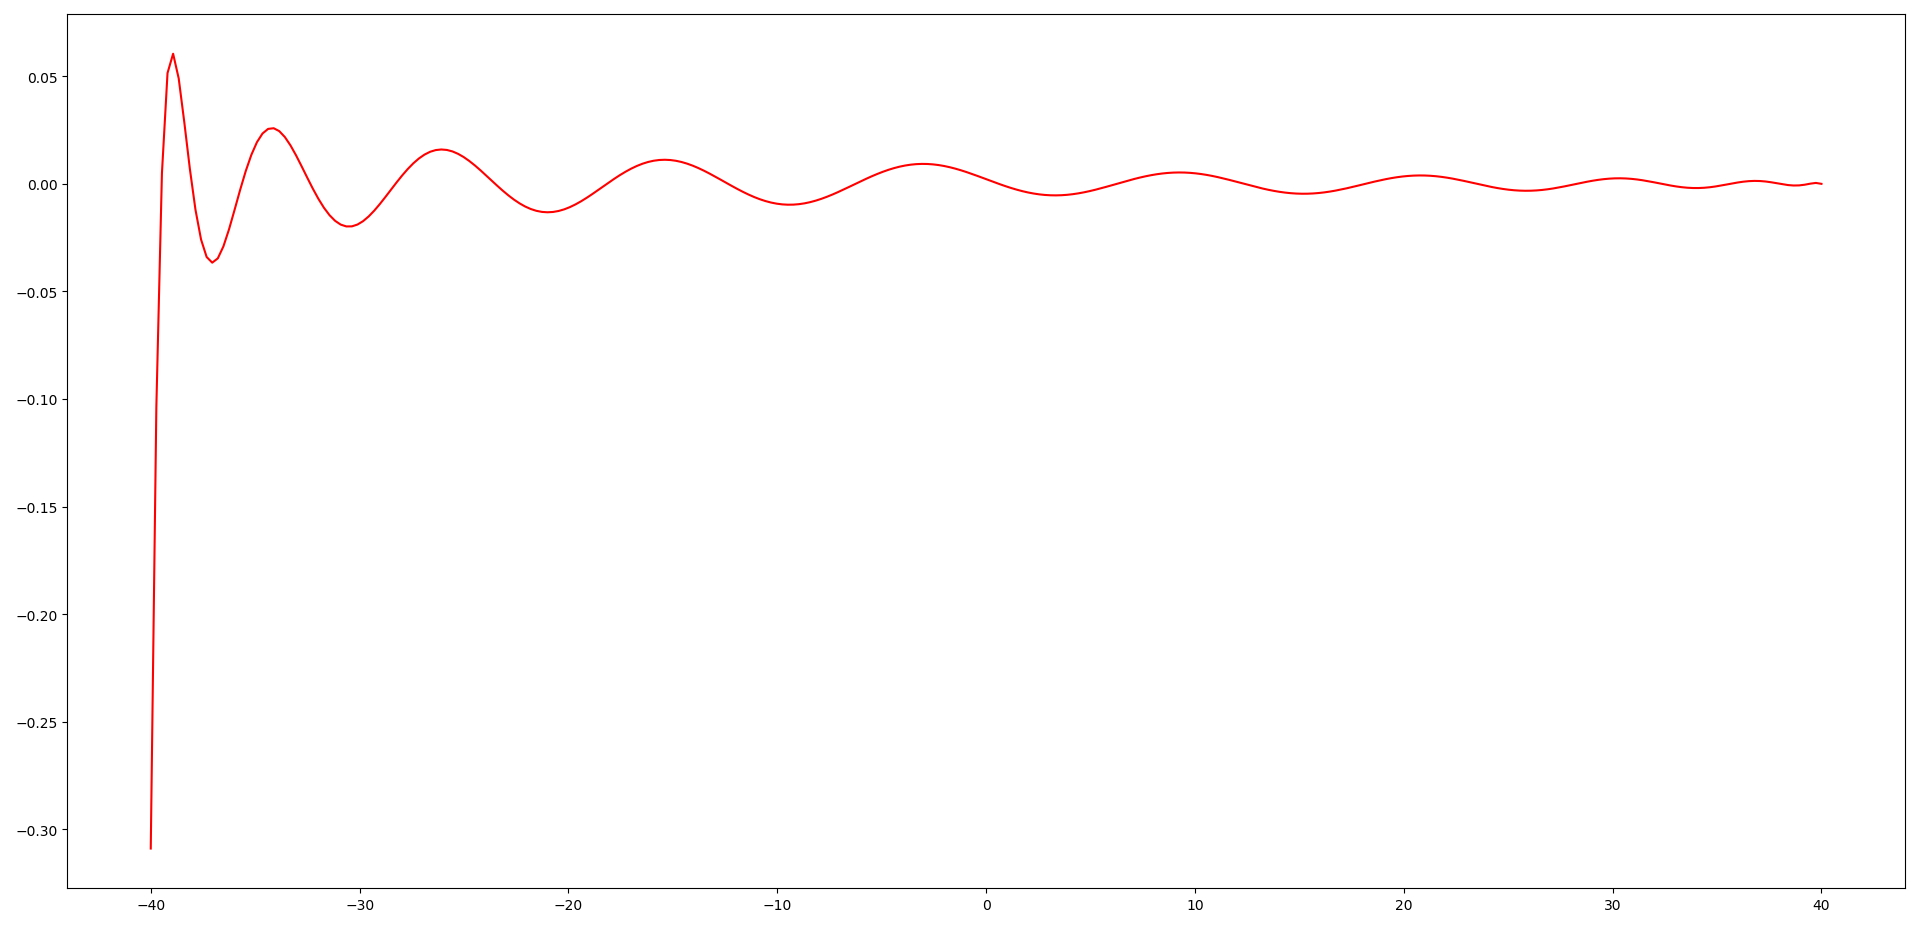
\includegraphics[scale=0.38]{solution_unlabeled}
	\caption{$x$ vs. $y(x)$}
\end{figure}
\end{landscape}
\end{document}










